% EF5342 Week 3 — Bond Markets and Bond Pricing
% Beamer conversion from week3_BondMarket.pptx (60 source slides -> 41 frames).
% Compile: pdflatex week3_BondMarket.tex
% Each frame carries a [src: ...] comment mapping back to source slides.
\documentclass[aspectratio=169]{beamer}
\usepackage{../ef5342}

\title{EF5342 Financial Systems, Markets and Instruments}
\subtitle{Week 3 --- Bond Markets and Bond Pricing}
\author{Prof.\ Weikai Li}
\institute{City University of Hong Kong}
\date{Semester B 2026--2027}

\begin{document}

% ============ INTRODUCTION ============

% [src: 1]
\begin{frame}
\titlepage
% Title-page background image (slide01_img.jpg) dropped — decorative.
\end{frame}

% [src: 2]
\begin{frame}{Bond Markets and Bond Pricing}
\begin{itemize}
  \item Bond characteristics
  \item Treasury bonds, Munis, and corporate bonds
  \item Bond pricing and yield to maturity
  \item Interest rate risk and duration
\end{itemize}
\end{frame}

% [src: 3]
\begin{frame}{Fixed-Income Securities}
\begin{description}
  \item[Fixed-income security] (a.k.a.\ debt security, bond) promises a fixed stream of income, or a stream determined by a pre-specified formula
\end{description}
\vspace{0.2em}
\textbf{Key issues:}
\begin{itemize}
  \item How to value future payments (time value of money)
  \item Risk that the promise will not be kept (credit risk)
\end{itemize}
\vspace{0.2em}
\textbf{Two main payment streams:}
\begin{description}
  \item[Zero-coupon bonds] A single payment at maturity --- the face (par) value
  \item[Coupon bonds] Pay \$C each period (typically every six months) up to maturity, when they pay \$C $+$ face value
\end{description}
\note{Pre-specified formula allows for floating-rate bonds. The promise is not necessarily fulfilled. One dollar received at different points in the future should be worth differently now. In this class we won't deal with floating-rate bonds.}
\end{frame}

% [src: 4]
\begin{frame}{Fixed-Income Payoffs}
\begin{columns}
\begin{column}{0.54\textwidth}
\textbf{Zero-coupon bond:} nothing until $t+m$, then the face value (e.g., \$1,000).
\vspace{0.4em}

\textbf{Coupon bond:} \$C at $t+1$, \$C at $t+2$, \ldots, and \$C $+$ \$1{,}000 at maturity $t+m$.
\vspace{0.4em}

\textbf{Coupon rate} = \% of par value paid every coupon period, usually quoted annually; coupons can be paid more frequently.
\begin{itemize}
  \item Example: an 8\% semi-annual coupon bond pays \$40 every 6 months
\end{itemize}
\end{column}
\begin{column}{0.42\textwidth}
\begin{center}
\scriptsize
\begin{tabular}{lccccc}
\toprule
 & $t$ & $t{+}1$ & $t{+}2$ & $\cdots$ & $t{+}m$ \\
\midrule
Zero & & & & & 1{,}000 \\
Coupon & & $C$ & $C$ & $\cdots$ & $1{,}000+C$ \\
\bottomrule
\end{tabular}
\end{center}
\end{column}
\end{columns}
\note{Usually use the face value of \$1,000 as convention.}
\end{frame}

% [src: 5]
\begin{frame}{Coupon Bonds}
Before electronic registration, bonds were issued as physical certificates with detachable coupons --- every six months the holder tore off one coupon in exchange for the interest payment.
\begin{columns}
\begin{column}{0.42\textwidth}
\begin{figure}
\centering
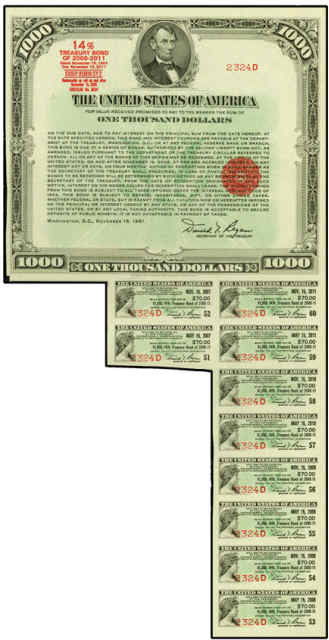
\includegraphics[height=0.58\textheight,keepaspectratio]{figures/slide05_img.png}
\end{figure}
\end{column}
\begin{column}{0.28\textwidth}
\begin{figure}
\centering
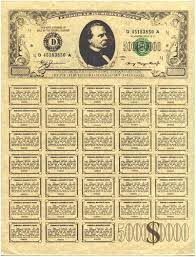
\includegraphics[height=0.42\textheight,keepaspectratio]{figures/slide05_img1.png}
\end{figure}
\end{column}
\end{columns}
\note{Every six months tear off one coupon in exchange for the interest payment.}
\end{frame}

% [src: 6, 7]
\begin{frame}{Major Types of Bonds}
Bonds are long-term debt obligations issued by corporations and governments (or government agencies):
\small
\begin{itemize}
  \item Treasury notes (T-notes) and bonds (T-bonds)
  \item Municipal bonds (Munis)
  \item Corporate bonds (investment-grade and high-yield)
  \item Mortgage-backed securities (MBS) and asset-backed securities (ABS)
\end{itemize}
\begin{columns}
\begin{column}{0.50\textwidth}
\begin{figure}
\centering

\includegraphics[width=0.72\linewidth,keepaspectratio]{figures/slide06_img_flat.png}
\end{figure}
\end{column}
\begin{column}{0.46\textwidth}
\begin{figure}
\centering
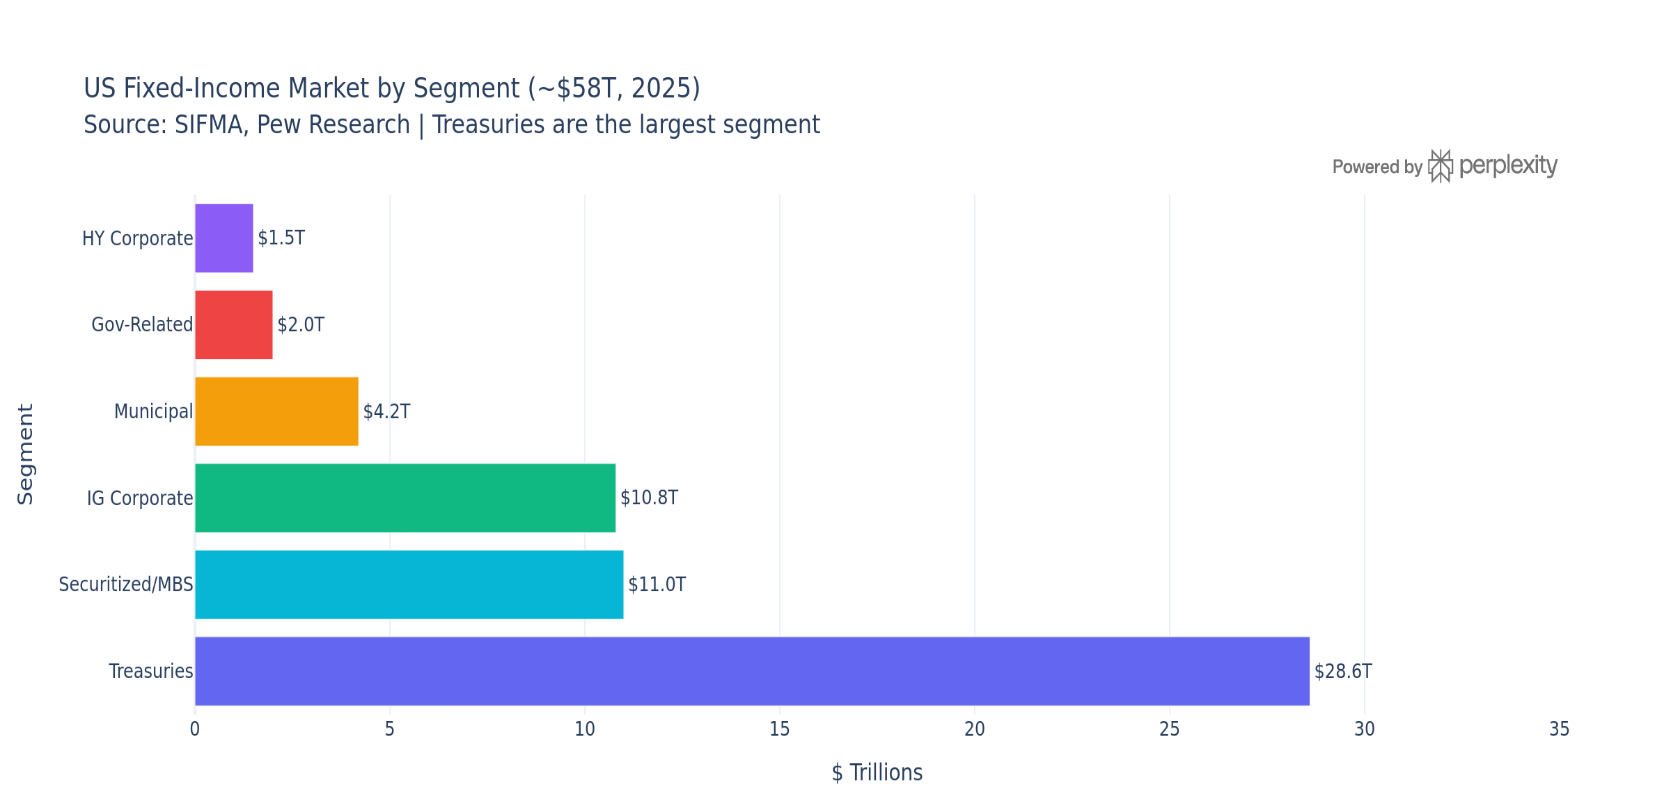
\includegraphics[width=0.72\linewidth,keepaspectratio]{figures/slide07_img1_flat.png}
\end{figure}
\end{column}
\end{columns}
\note{T-bonds are issued by the federal government; municipal bonds by state and local governments.}
\end{frame}

% ============ TREASURY / MUNI / CORPORATE ============

% [src: 8]
\section{Treasury Bonds, Munis, and Corporate Bonds}

% [src: 9]
\begin{frame}{Treasury Notes and Bonds}
Issued by the U.S.\ Treasury to finance the national debt and other government expenditures.
\begin{itemize}
  \item \textbf{Default-risk free:} backed by ``full faith and credit'' of the U.S.\ federal government
  \item \textbf{Low returns:} low interest rates reflect minimum default risk
  \item \textbf{Interest rate risk:} longer maturity $\Rightarrow$ wider price fluctuations than T-bills when rates change
  \item \textbf{Liquidity risk:} very active secondary markets, but older (``off-the-run'') issues are less liquid than newly issued (``on-the-run'') ones
  \item \textbf{Inflation risk:} inflation may erode the purchasing power of future nominal payments
\end{itemize}
\vspace{0.2em}
T-notes: original maturities of 2, 3, 5, 7, and 10 years; T-bonds: $>$ 10 years. Prices are quoted as a percentage of par (usually \$1,000).
\note{Newly issued Treasuries are called on-the-run; older Treasuries off-the-run.}
\end{frame}

% [src: 10]
\begin{frame}{Interest Rate Risk: Treasury Bonds vs.\ Notes}
The total-return index of Treasury \textbf{bonds} with 20+ years of maturity (blue) is much more volatile than Treasury \textbf{notes} with 3--7 years of maturity (orange).
\begin{figure}
\centering
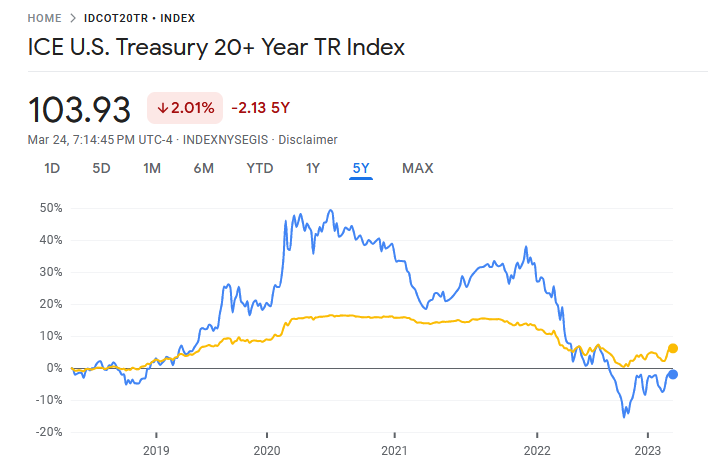
\includegraphics[height=0.60\textheight,keepaspectratio]{figures/slide10_img_flat.png}
\end{figure}
\begin{center}\small Source: Google Finance\end{center}
\end{frame}

% [src: 11]
\begin{frame}{Major Foreign Holders of U.S.\ Treasury Securities}
As of June 2026, Japan is the largest foreign holder of U.S.\ Treasury securities (\$1{,}116 billion), followed by the United Kingdom (\$940 billion) and China (\$633 billion --- its lowest level since 2008); total foreign holdings are \$9.29 trillion (Treasury TIC). The U.K.\ has overtaken China as the second-largest holder.
\begin{figure}
\centering
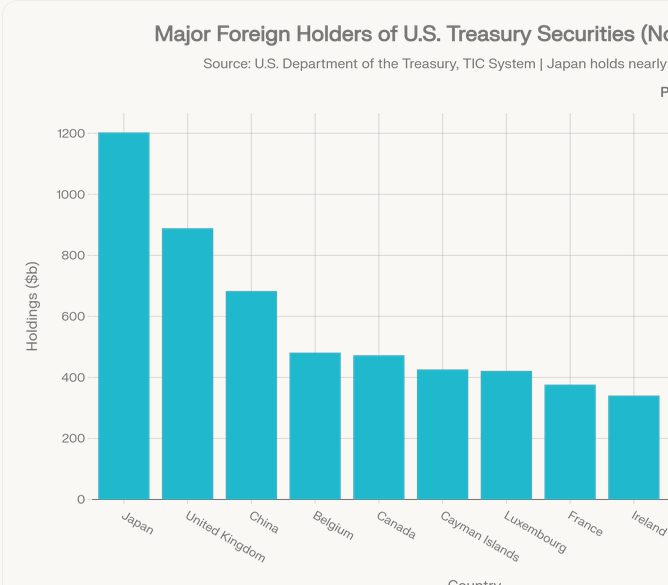
\includegraphics[height=0.56\textheight,keepaspectratio]{figures/slide11_img_flat.png}
\end{figure}
\end{frame}

% [src: 12, 13]
\begin{frame}{Accrued Interest}
\textbf{Accrued interest} is the portion of the coupon payment accrued between the last coupon payment and the settlement date. It must be paid by the \emph{buyer} of a bond to the \emph{seller} if the bond is purchased between coupon payment dates.
\begin{columns}
\begin{column}{0.52\textwidth}
\begin{figure}
\centering
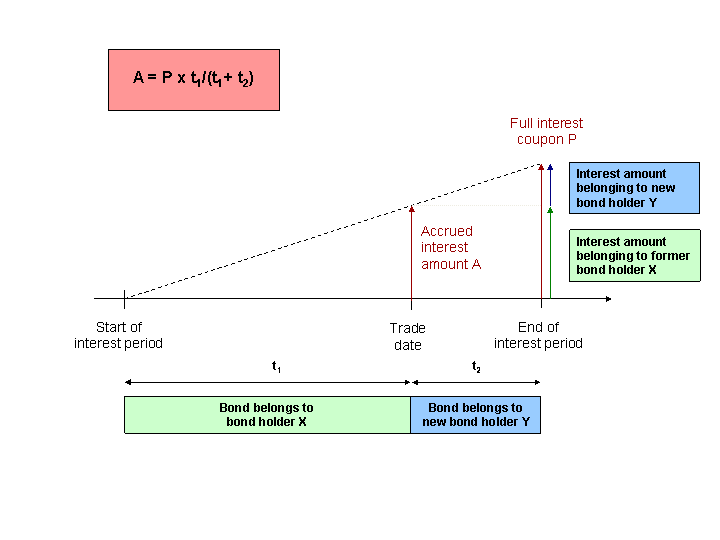
\includegraphics[height=0.46\textheight,width=\linewidth,keepaspectratio]{figures/slide12_img_conv.png}
\end{figure}
\end{column}
\begin{column}{0.44\textwidth}
\begin{figure}
\centering

\includegraphics[height=0.46\textheight,width=\linewidth,keepaspectratio]{figures/slide13_img_flat.png}
\end{figure}
\end{column}
\end{columns}
\end{frame}

% [src: 14]
\begin{frame}{Accrued Interest: Example}
You buy a 6\% coupon \$1{,}000-par T-bond 59 days after the last coupon payment; settlement occurs in two days, so you become the owner \textbf{61 days} after the last coupon, with \textbf{121 days} remaining until the next coupon. The bond's flat price is quoted at 120.593. What is the invoice price?
\vspace{0.4em}
\begin{itemize}
  \item Flat price: $120.593\% \times \$1{,}000 = \$1{,}205.93$
  \item Accrued interest: $\frac{61}{61+121} \times \$30 = \$10.05$
  \item Invoice price: $\$1{,}205.93 + \$10.05 = \mathbf{\$1{,}215.98}$
\end{itemize}
\vspace{0.4em}
\begin{figure}
\centering

\includegraphics[width=0.78\textwidth,keepaspectratio]{figures/slide14_img_flat.png}
\end{figure}
\end{frame}

% [src: 15, 16]
\begin{frame}{Treasury Inflation-Protected Securities (TIPS)}
TIPS protect investors against inflation by adjusting the bond's \textbf{principal daily} based on changes in the CPI-U. The coupon rate is fixed --- but applied to the inflation-adjusted principal, so coupons rise with inflation.
\begin{itemize}
  \item Example: \$1{,}000 par, 3\% coupon, 10\% inflation $\Rightarrow$ principal adjusts to \$1{,}100; coupon becomes $3\% \times \$1{,}100 = \$33$ rather than \$30
  \item TIPS provide a \textbf{real} yield; nominal Treasuries a nominal yield
  \item At maturity, investors receive the \emph{greater} of adjusted principal or original face --- deflation protection
\end{itemize}
\vspace{0.2em}
\textbf{Decomposition:} Nominal Treasury yield $=$ TIPS real yield $+$ breakeven inflation rate. Expected inflation turned negative in the 2008 GFC period.
\begin{figure}
\centering

\includegraphics[height=0.25\textheight,width=0.86\textwidth,keepaspectratio]{figures/slide16_img_flat.png}
\end{figure}
\end{frame}

% [src: 17]
\begin{frame}{How the Treasury Market Works}
The U.S.\ Treasury conducts regular auctions through TAAPS. Three types of bidders:
\begin{description}
  \item[Primary dealers] 24 designated counterparties (e.g., JPMorgan, Goldman Sachs, Citi), required to bid at all auctions at reasonably competitive prices --- market-makers of last resort
  \item[Direct bidders] Institutional investors (pension funds, central banks) accessing auctions directly through TAAPS
  \item[Indirect bidders] Foreign official institutions and investors routing through intermediaries --- often read as a proxy for foreign central bank demand
\end{description}
\vspace{0.2em}
The secondary market is an OTC dealer market with primary dealers quoting bid--ask spreads; average daily trading volume was roughly \$1.0 trillion in 2025 (SIFMA, up 16\% year-over-year) --- the world's most liquid market.
\end{frame}

% [src: 18]
\begin{frame}{Historical Returns of U.S.\ Treasury Bonds}
\textbf{2022 was catastrophic:} $-14.36\%$ total return for U.S.\ Treasuries --- the worst single year in modern U.S.\ bond market history. The Bloomberg U.S.\ Aggregate fell $-13.01\%$. This reflected the fastest tightening cycle since the 1980s. Returns were positive again in 2025 amid historically tight credit spreads.
\begin{figure}
\centering

\includegraphics[height=0.60\textheight,keepaspectratio]{figures/slide18_img_flat.png}
\end{figure}
\end{frame}

% [src: 19]
\begin{frame}{Fiscal Dynamics and the Bond Market}
The U.S.\ federal deficit reached \textbf{\$1.78 trillion in fiscal year 2025 (5.9\% of GDP)}; debt held by the public stood near 99.8\% of GDP, and net interest exceeded \$1 trillion for the first time (CBO). These dynamics affect yields through two channels:
\begin{description}
  \item[Supply effect] Persistent large issuance requires the market to absorb more Treasury supply; if demand does not scale proportionally, yields must rise to attract buyers
  \item[Term-premium channel] Fiscal uncertainty raises the risk premium investors demand for holding long-duration government bonds --- lifting long-end yields independently of policy-rate expectations
\end{description}
\begin{figure}
\centering
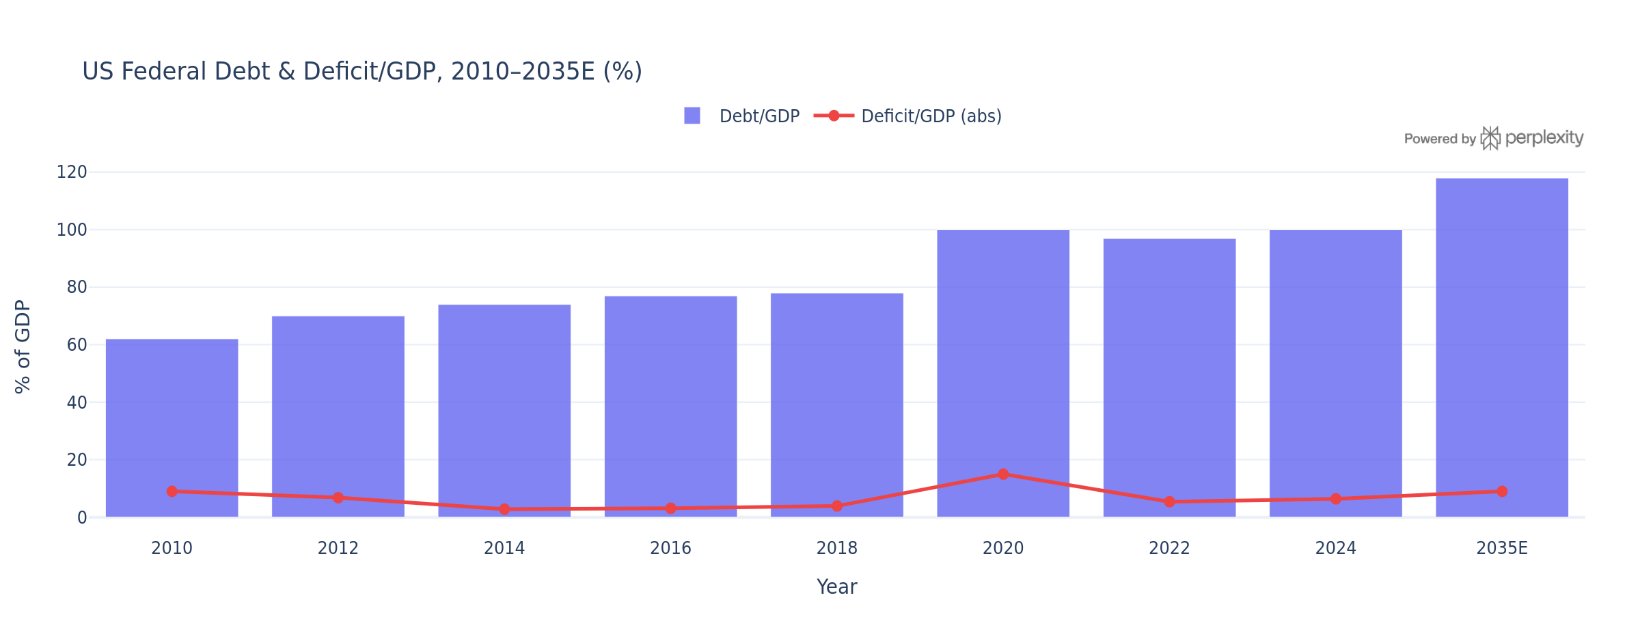
\includegraphics[height=0.34\textheight,width=0.9\textwidth,keepaspectratio]{figures/slide19_img_flat.png}
\end{figure}
\end{frame}

% [src: 20]
\begin{frame}{Municipal Bonds}
Debt securities issued by state and local governments to finance long-term projects (roads, schools, airports\ldots). Attractive because interest income on most Munis is \textbf{exempt from federal income tax} (and often from state and local taxes for in-state residents).
\vspace{0.3em}
\begin{description}
  \item[General obligation (GO) bonds] Backed by the full faith and credit of the issuing municipality
  \item[Revenue bonds] Sold to finance specific revenue-generating projects
\end{description}
\vspace{0.3em}
\textbf{Question:} which type is riskier?
\note{The majority of Munis are revenue bonds.}
\end{frame}

% [src: 21, 22]
\begin{frame}{Municipal Bond Yields}
Because Munis are tax-exempt, compare after-tax yields. For a corporate bond:
\[
i_a = i_b(1 - t)
\qquad\text{where } i_a = \text{after-tax yield},\quad i_b = \text{before-tax yield},\quad t = \text{marginal tax rate}
\]
Equivalently, convert the Muni yield to an equivalent before-tax yield: $i_b = i_a/(1-t)$.
\vspace{0.4em}
\textbf{Examples (28\% tax bracket):}
\begin{itemize}
  \item After-tax yield of a 6\% corporate yield: $i_a = 6\% \times (1-0.28) = \mathbf{4.32\%}$
  \item Corporate yield equivalent to a 4.5\% Muni: $i_b = 4.5\%/(1-0.28) = \mathbf{6.25\%}$
\end{itemize}
\end{frame}

% [src: 23]
\begin{frame}{Corporate Bonds}
Long-term debt obligations issued by corporations; most trade over-the-counter in a network of bond dealers. Listings include issuer name, coupon rate, maturity date, price, yield, and credit ratings.
\begin{columns}
\begin{column}{0.54\textwidth}
\begin{figure}
\centering
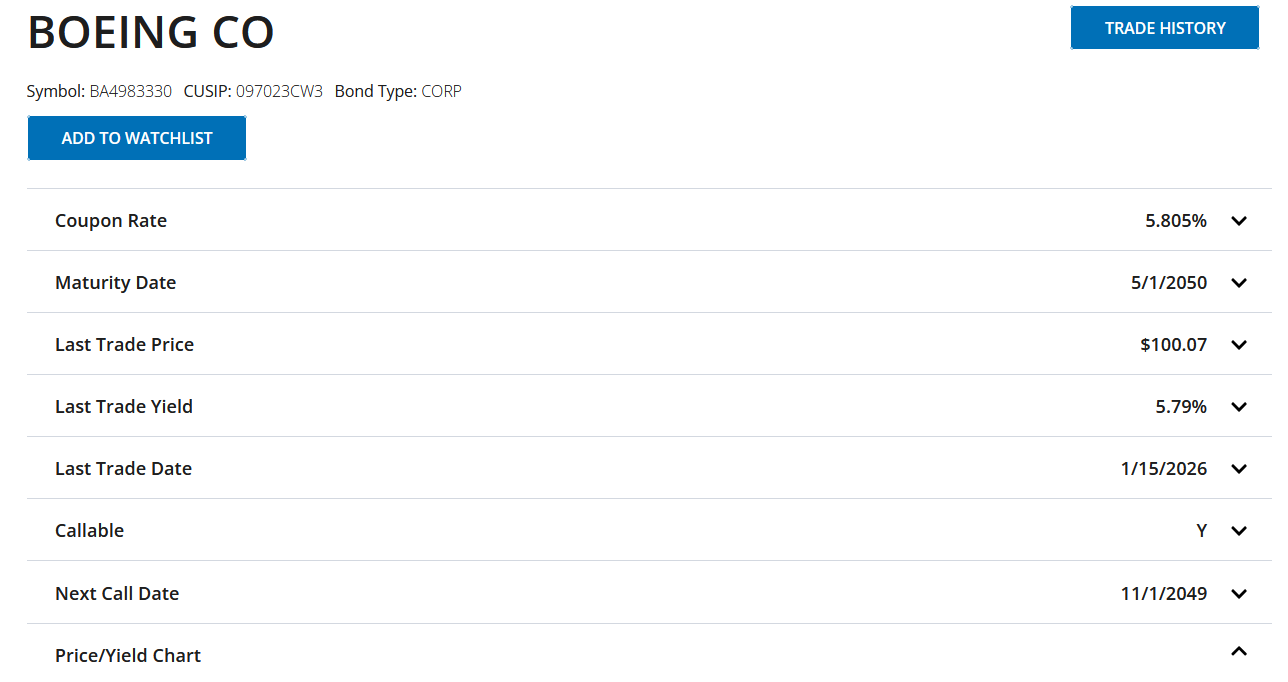
\includegraphics[width=\linewidth,keepaspectratio]{figures/slide23_img_flat.png}
\end{figure}
\end{column}
\begin{column}{0.42\textwidth}
\begin{figure}
\centering
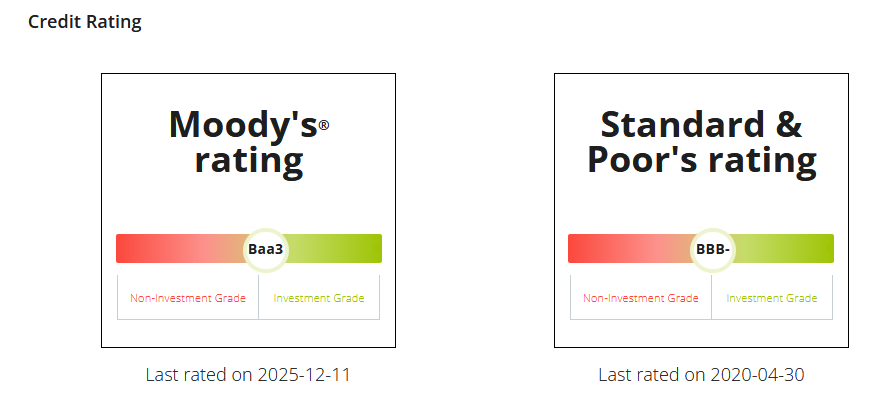
\includegraphics[width=\linewidth,keepaspectratio]{figures/slide23_img1_flat.png}
\end{figure}
\end{column}
\end{columns}
\note{Example listing: FINRA bond market data (\url{https://www.finra.org/finra-data/fixed-income/bond}).}
\end{frame}

% [src: 24, 25]
\begin{frame}{Bond Prices and Yields: An Inverse Relationship}
\begin{columns}
\begin{column}{0.46\textwidth}
\begin{figure}
\centering

\includegraphics[width=\linewidth,keepaspectratio]{figures/slide24_img_flat.png}
\end{figure}
\end{column}
\begin{column}{0.50\textwidth}
\textbf{Convertible bonds} give holders an option to exchange each bond for a specified number of common shares of the issuer.
\begin{itemize}
  \item Example: a \$1{,}000-par convertible exchangeable into 40 shares (stock at \$20): converting now yields $40 \times \$20 = \$800 <$ par --- not profitable now; profitable once the stock rises above \$25
  \item The option is valuable $\Rightarrow$ convertibles offer \emph{lower} yields than comparable non-convertibles
\end{itemize}
\end{column}
\end{columns}
\end{frame}

% [src: 26, 27]
\begin{frame}{Callable Bonds}
A \textbf{call provision} lets the issuer repurchase the bond at a pre-specified (call) price after a certain time.
\begin{itemize}
  \item Bonds are usually called when interest rates \emph{drop}, so the issuer can refinance at lower rates
  \item Bondholders dislike calls --- they must reinvest at lower rates $\Rightarrow$ callable bonds offer \emph{higher} yields than comparable non-callables
  \item The callable bond's value is \textbf{capped by the call price} as interest rates decrease
\end{itemize}
\begin{columns}
\begin{column}{0.52\textwidth}
\begin{figure}
\centering

\includegraphics[height=0.44\textheight,keepaspectratio]{figures/slide27_img.png}
\end{figure}
\end{column}
\begin{column}{0.42\textwidth}
\small Corporate bonds without options attached are called \textbf{straight bonds}.
\end{column}
\end{columns}
\end{frame}

% [src: 28, 29]
\begin{frame}{Credit Risk and Bond Ratings}
Are coupons/par guaranteed? \textbf{No} --- default is possible. Recent defaults: Enron, WorldCom, Lehman; sovereigns Russia (1998), Argentina (2001), Greece (2012); USD bonds of China property developers like Evergrande (2021).
\vspace{0.2em}
Three major rating agencies: \textbf{Moody's, S\&P, Fitch}. Bonds are rated by perceived default risk and categorized as \textbf{investment grade} or \textbf{speculative grade} (junk / high-yield).
\begin{itemize}
  \item Speculative grade $\Rightarrow$ higher default probability, compensated by higher yields
  \item \textbf{Fallen angel:} downgraded from IG to HY; \textbf{rising star:} upgraded HY to IG (expanded buyer base)
\end{itemize}
\begin{figure}
\centering
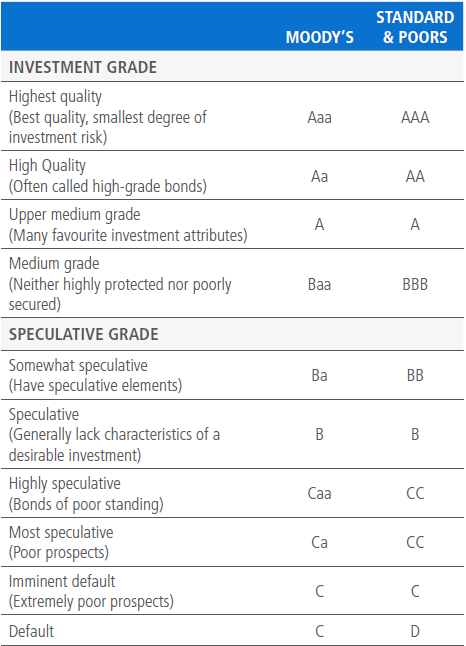
\includegraphics[height=0.36\textheight,keepaspectratio]{figures/slide29_img.PNG}
\end{figure}
\end{frame}

% ============ PRICING ============

% [src: 30]
\section{Bond Pricing and Yield to Maturity}

% [src: 31, 32]
\begin{frame}{Bond Pricing}
A bond's value is the sum of the present values of its future payment streams. Three components: future cash flows, the interest rate (discount rate), and price (present value).
\vspace{0.3em}
\textbf{Zero-coupon bond:}
\[
P = \frac{FV}{(1+r)^T}
\]
\textbf{Coupon bond} (pays \$C each period for $T$ periods):
\[
P = \sum_{t=1}^{T} \frac{C}{(1+r)^t} + \frac{FV}{(1+r)^T}
\]
where $r$ is the discount rate investors require to hold the bond. Coupon rates and $r$ are quoted \emph{annually} (APR convention); most bonds pay coupons semi-annually.
\note{For now take $r$ as given: the rate of return investors require to hold the bond; with abuse of terminology we also call it the interest rate in this lecture. A zero-coupon bond is the special case $C=0$. Ask students: which would have the higher interest rate --- a 3-year bond or a 100-year bond; a Treasury bond or a corporate bond?}
\end{frame}

% [src: 33, 34]
\begin{frame}{Semi-Annual Compounding}
With semi-annual coupons, adjust both the payment and the discount rate. One dollar grows to:
\[
\$\left(1+\tfrac{r}{2}\right) \text{ after 6 months},\qquad
\$\left(1+\tfrac{r}{2}\right)^{2} \text{ after 1 year},\qquad
\$\left(1+\tfrac{r}{2}\right)^{2T} \text{ after } T \text{ years}
\]
\vspace{0.2em}
So the semi-annual bond pricing formula (coupon halved to $C/2$, discount rate $r/2$, $2T$ payments):
\[
P = \sum_{t=1}^{2T} \frac{C/2}{\left(1+\frac{r}{2}\right)^{t}} + \frac{FV}{\left(1+\frac{r}{2}\right)^{2T}}
\]
\note{The semi-annual discount rate is r/2. Do not forget the coupon payment is also halved (every six months you get C/2); adjust the discount rate; remember you now have 2T payments.}
\end{frame}

% [src: 35, 36]
\begin{frame}{Bond Pricing: Example}
Price a bond that pays a \textbf{10\% coupon} and matures in \textbf{12 years}; the interest rate is \textbf{8\%}. (Unstated face value is \$1{,}000 by convention.)
\begin{itemize}
  \item Too many coupons to add up one by one --- use the annuity formula:
  $\displaystyle\sum_{t=1}^{T}\frac{C}{(1+r)^t} = \frac{C}{r}\left[1-\frac{1}{(1+r)^T}\right]$
  \item Semi-annual coupon bond: $r \to 4\%$, $T \to 24$ periods, $C \to \$50$:
\end{itemize}
\[
P = \frac{50}{0.04}\left(1-\frac{1}{1.04^{24}}\right) + \frac{1000}{(1+0.04)^{24}} = \$1{,}152.47
\]
\vspace{0.3em}
\textbf{Excel:} \texttt{=PV(0.04, 24, 50, 1000)} \quad \textbf{Financial calculator:} $I=4$, $PMT=50$, $FV=1000$, $T=24 \Rightarrow PV = -1152.47$
\note{Negative PV because buying the bond is a cash outflow.}
\end{frame}

% [src: 37, 38, 39]
\begin{frame}{Interest Rates and Bond Prices}
Same 10\%-coupon, 12-year bond at different required rates:
\[
r = 12\%: \quad P = \frac{50}{0.06}\left(1-\frac{1}{1.06^{24}}\right) + \frac{1000}{1.06^{24}} = \$874.50
\qquad
r = 10\%: \quad P = \$1{,}000 \ (\text{par})
\]
\begin{center}
\begin{tabular}{ccc}
\toprule
Interest rate & Bond price & \\
\midrule
12\% & 874.50 & discount \\
10\% & 1{,}000 & par \\
8\% & 1{,}152.47 & premium \\
\bottomrule
\end{tabular}
\end{center}
\textbf{VERY important:}
\begin{itemize}
  \item \textbf{Inverse relationship} between bond price and interest rate (if $r$ falls, $P$ rises)
  \item The price--rate relationship is \textbf{non-linear} (convex)
  \item \textbf{Premium bond:} $C > r \Rightarrow V_b > \text{Par}$; \textbf{discount bond:} $C < r \Rightarrow V_b < \text{Par}$; \textbf{par bond:} $C = r \Rightarrow V_b = \text{Par}$
\end{itemize}
\end{frame}

% [src: 40]
\begin{frame}{Yield to Maturity}
\begin{description}
  \item[Yield to maturity (YTM)] The interest rate $y$ at which the bond's present value equals its price --- the bond's IRR
\end{description}
\vspace{0.2em}
Roughly, the average annual return from buying at the market price and holding to maturity. For semi-annual bonds, solve:
\[
P = \sum_{t=1}^{2T} \frac{C/2}{\left(1+\frac{y}{2}\right)^{t}} + \frac{FV}{\left(1+\frac{y}{2}\right)^{2T}}
\]
Calculable in Excel or with a financial calculator.
\note{Let's flip the table. In calculating the price, investors know the future cash flows and have a secret sheet with interest rates. Now assume you are an outsider: you know the cash flows but not the discount rate. What you can observe is the price at which the bond trades --- you back out the discount rate.}
\end{frame}

% [src: 41]
\begin{frame}{Yield to Maturity: Example}
Consider a semi-annual bond: $T=2$ years, $C=\$20$ per period, $P=909.2$, $FV=\$1{,}000$. Solve:
\[
909.2 = \sum_{t=1}^{4} \frac{20}{\left(1+\frac{y}{2}\right)^{t}} + \frac{1000}{\left(1+\frac{y}{2}\right)^{4}}
\quad\Longrightarrow\quad y = \mathbf{6.94\%} \ \text{(annualized)}
\]
\end{frame}

% [src: 42]
\begin{frame}{What Factors Affect Bond Yields?}
\begin{description}
  \item[Default risk] The most important factor: higher default risk $\Rightarrow$ investors require higher yields
  \item[Maturity] Longer-maturity bonds are more sensitive to rate changes, so typically have higher yields
  \item[Liquidity] Less liquid bonds pay higher yields to compensate for trading costs
  \item[Convertibility] Convertibles have \emph{lower} yields --- investors get the valuable conversion option
  \item[Callability] Calls are typically exercised when rates fall $\Rightarrow$ investors demand higher yields on callable bonds
\end{description}
\end{frame}

% [src: 43, 44]
\begin{frame}{Credit Spreads}
Corporations have larger default risk and higher yields than Treasuries of similar maturity --- creating a \textbf{credit spread}.
\begin{itemize}
  \item Historically, IG spreads average $\sim$130 basis points; HY spreads $\sim$450 bps
  \item COVID shock (March 2020): IG spreads jumped to $\sim$372 bps, HY to over 1{,}000 bps before central-bank intervention compressed them; as of end-August 2026 spreads remain historically tight (HY OAS 2.63\% vs.\ a long-run average near 475 bps)
\end{itemize}
\begin{figure}
\centering
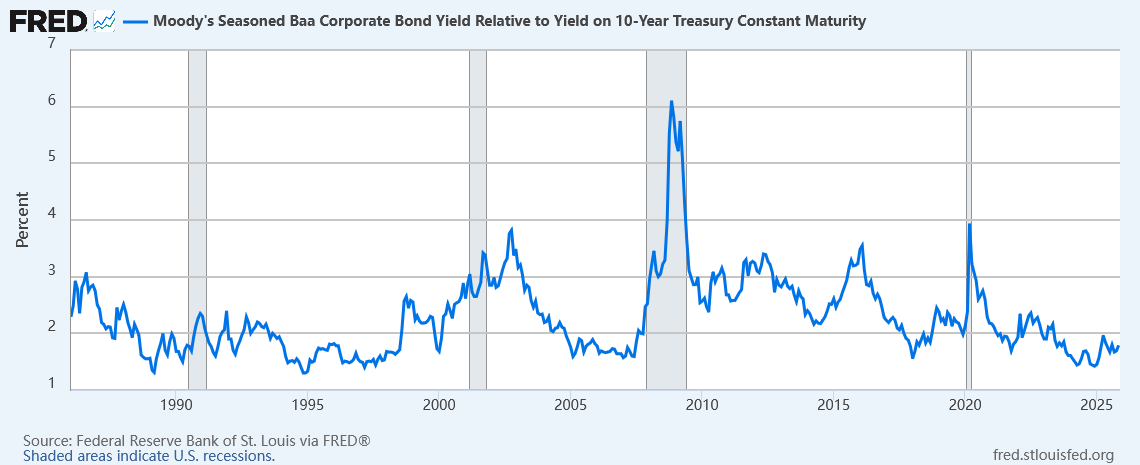
\includegraphics[height=0.44\textheight,keepaspectratio]{figures/slide44_img_flat.png}
\end{figure}
\note{The industry-standard measure is the option-adjusted spread (OAS), which strips out embedded options to isolate the pure credit spread.}
\end{frame}

% ============ INTEREST RATE RISK ============

% [src: 45]
\section{Interest Rate Risk and Duration}

% [src: 46, 47]
\begin{frame}{Interest Rate Risk}
Bond prices are sensitive to interest rates:
\begin{itemize}
  \item \textbf{Inverse relationship:} rates rise $\Rightarrow$ prices fall (rising rates are bad news for bond investors)
  \item The relationship is \textbf{convex}, not linear --- but for small changes a linear approximation works
  \item \textbf{Long-term} bonds are more sensitive than short-term (the coupon is locked in for longer)
  \item \textbf{Higher-coupon} bonds pay more cash flow early, so they are less sensitive
\end{itemize}
We want a measure of ``how long-term'' a bond is that captures both maturity and coupon effects.
\begin{figure}
\centering

\includegraphics[height=0.30\textheight,keepaspectratio]{figures/slide46_img.png}
\end{figure}
\note{With very small changes we can approximate the convex relationship with a linear one. For higher-coupon bonds you get back a greater fraction of value in the interim and can reinvest at the prevailing rate.}
\end{frame}

% [src: 48, 49]
\begin{frame}{Duration}
\textbf{Duration} measures the average maturity of a bond's promised cash flows: the weighted average of times to each coupon or principal payment, where the weight on each payment time is the proportion of bond value it accounts for.
\[
D = \sum_{t=1}^{T} t \cdot w_t,
\qquad
w_t = \frac{CF_t/(1+y)^t}{P}, \qquad \sum_t w_t = 1
\]
where $P$ = bond price, $CF_t$ = cash flow at end of period $t$, $y$ = yield to maturity.
\note{If the security makes semiannual or monthly payments, the cash flows, interest rate, and number of periods must be adjusted to the payment frequency.}
\end{frame}

% [src: 50, 51]
% NOTE: source slides also carry EMF tables (the headline 3.6793/3.8213-year
% duration results) that could not be rasterized; only the Part 1/Part 2
% calculation PNGs are shown. Results stated below are from the slide text.
\begin{frame}{Duration: Examples 1 and 2}
\begin{columns}
\begin{column}{0.48\textwidth}
\begin{figure}
\centering
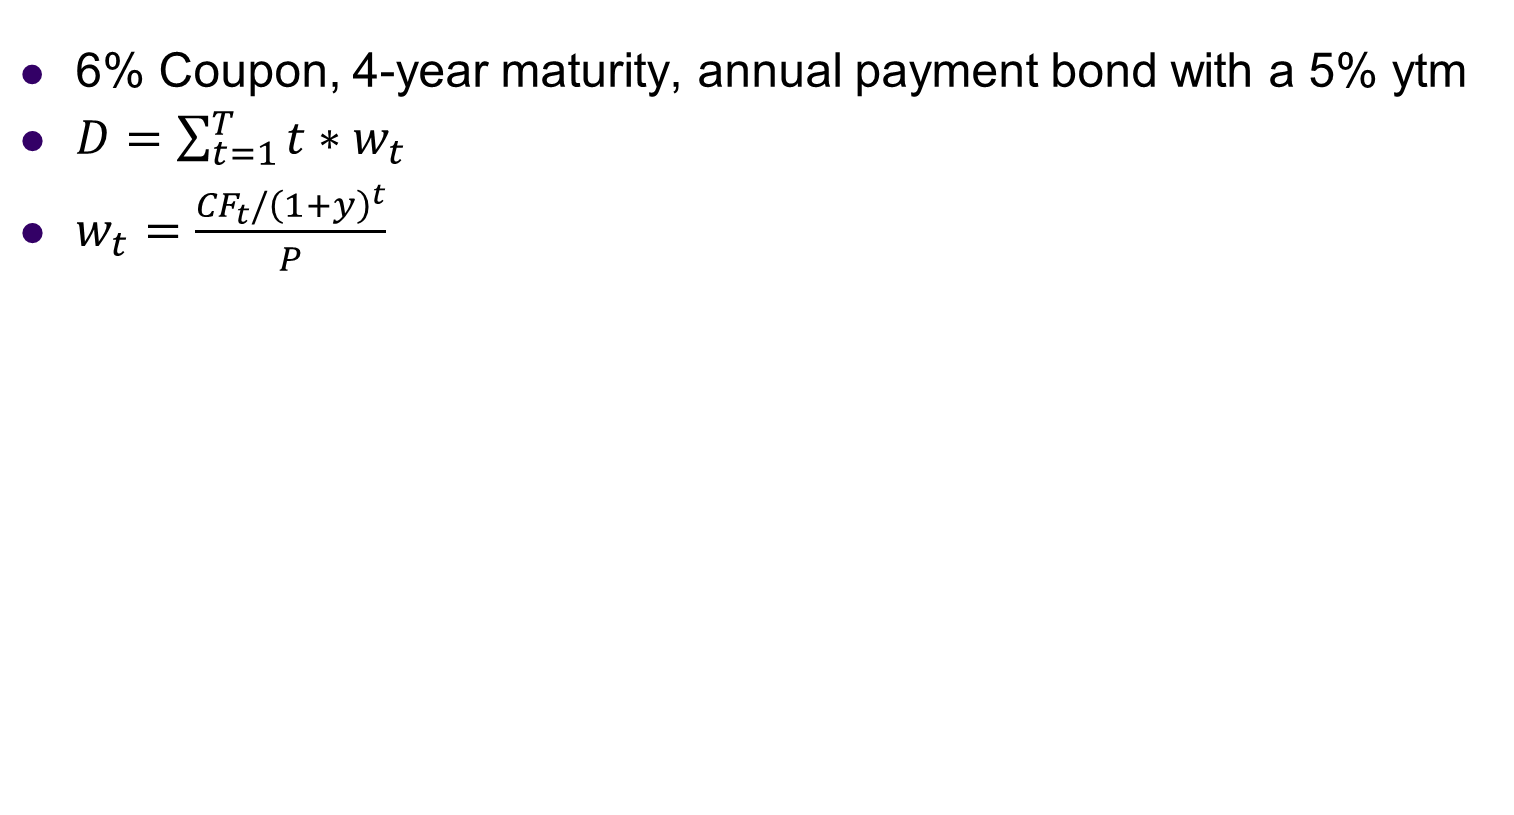
\includegraphics[width=\linewidth,keepaspectratio]{figures/slide50_img_flat.png}
\end{figure}
\end{column}
\begin{column}{0.48\textwidth}
\begin{figure}
\centering
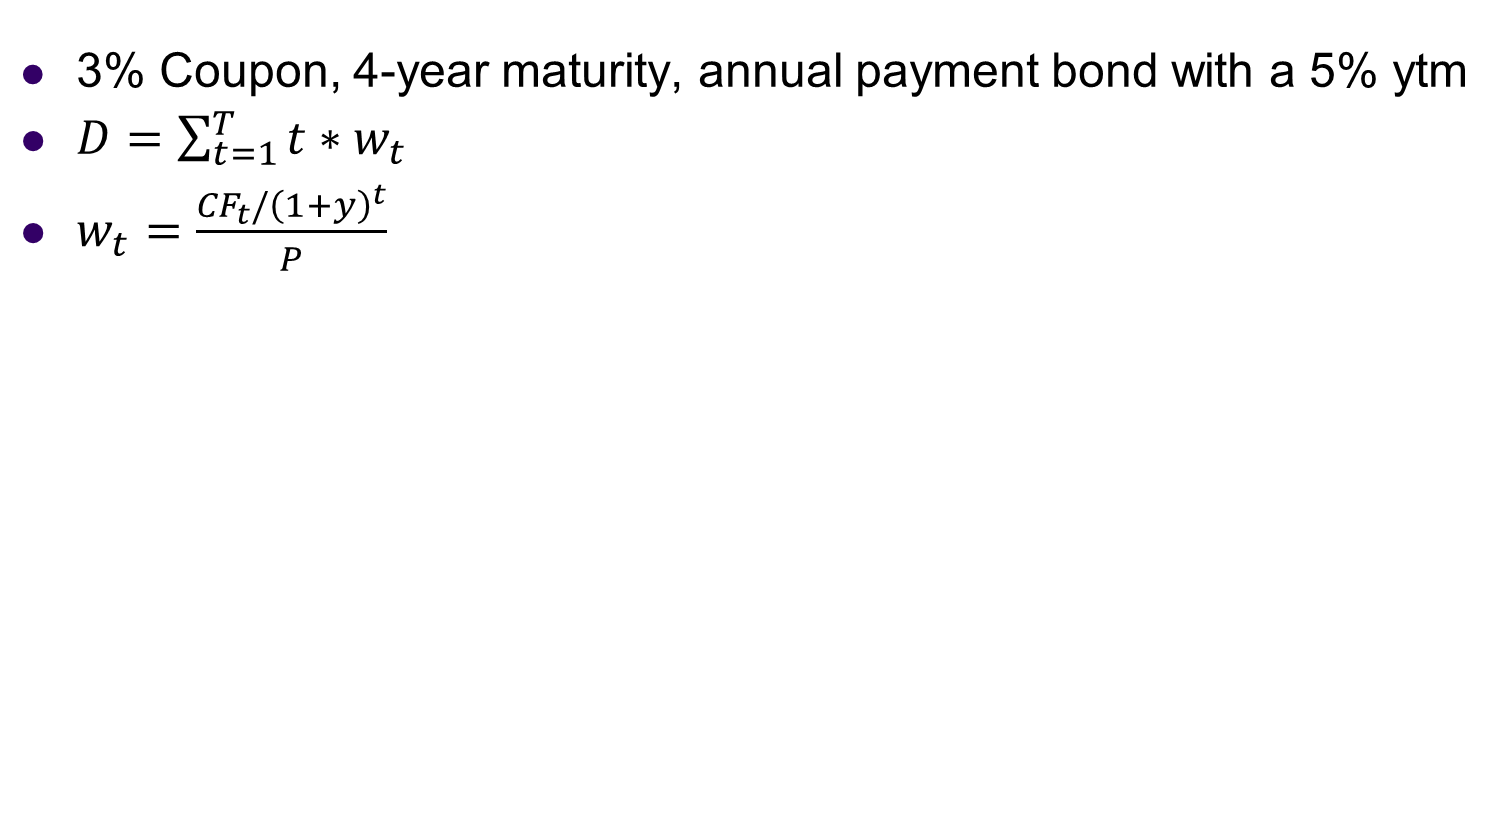
\includegraphics[width=\linewidth,keepaspectratio]{figures/slide51_img_flat.png}
\end{figure}
\end{column}
\end{columns}
\vspace{0.2em}
\small Worked calculation: Part 1 finds the present value of each cash flow; Part 2 takes the weighted average of payment times. Slide results: \textbf{Example 1:} $D = 3.6793$ years; \textbf{Example 2} (lower coupon): $D = 3.8213$ years.
\note{Example 1: same sensitivity as a zero maturing in 3.679 years. Example 2: with a lower coupon the bond has longer duration and larger price volatility --- a lower percentage of the investment is returned in the early years.}
\end{frame}

% [src: 52]
\begin{frame}{Duration: Example 3}
\begin{columns}
\begin{column}{0.52\textwidth}
\begin{figure}
\centering

\includegraphics[width=\linewidth,keepaspectratio]{figures/slide52_img_flat.png}
\end{figure}
\end{column}
\begin{column}{0.42\textwidth}
Duration $= 5.2342$ years.
\vspace{0.4em}

With a \textbf{longer maturity}, duration is longer and price volatility larger. Of the two effects, \textbf{maturity is the predominant} determinant of duration.
\end{column}
\end{columns}
\note{This bond has approximately the interest rate sensitivity of a zero-coupon bond maturing in 5.234 years.}
\end{frame}

% [src: 53]
\begin{frame}{Duration of Zero-Coupon Bonds}
A zero-coupon bond makes a single payment, so its duration equals its maturity:
\[
D = 1 \times \frac{CF_1/(1+y)}{P} = T \qquad (\text{one payment at } T)
\]
E.g., a one-year zero: $D = 1 \cdot \frac{1000/1.10}{1000/1.10} = 1$.
\vspace{0.3em}
\begin{itemize}
  \item Coupon bonds always have $D < T$
  \item The higher the coupon rate, the more weight on early payments and the shorter the duration
\end{itemize}
\end{frame}

% [src: 54]
\begin{frame}{What Determines Bond Duration?}
\begin{description}
  \item[Coupon rate] Higher coupon $\Rightarrow$ \emph{shorter} duration: cash flows arrive earlier and carry higher weights in the calculation
  \item[Maturity] Longer maturity $\Rightarrow$ \emph{longer} duration: generalizes the idea that long-term bonds are more rate-sensitive than short-term bonds
  \item[Yield to maturity] Higher YTM $\Rightarrow$ \emph{shorter} duration: later cash flows are discounted more heavily, shrinking their weights
\end{description}
\end{frame}

% [src: 55, 56]
\begin{frame}{Duration and Interest Rate Risk}
Duration gives a linear approximation to the percentage price change:
\[
\frac{\Delta P}{P} \approx -\,D \times \frac{\Delta y}{1+y}
\]
\textbf{Example.} A 2-year bond with 12\% coupon at a 10\% yield has $D = 1.8859$ years. If rates rise from 10\% to 12\% ($\Delta y = 0.02$):
\[
\frac{\Delta P}{P} \approx -\,1.8859 \times \frac{0.02}{1.10} = -3.43\%
\]
\note{Note that the annual change in interest rates is plugged into the prediction model.}
\end{frame}

% [src: 57, 58]
\begin{frame}{Duration-Based Prediction Errors}
Duration predicts price changes accurately only for \textbf{small} rate changes; day to day it works quite well. But when rates move significantly --- e.g., Fed funds-rate adjustments --- predicted pricing errors become significant.
\begin{columns}
\begin{column}{0.52\textwidth}
\begin{figure}
\centering
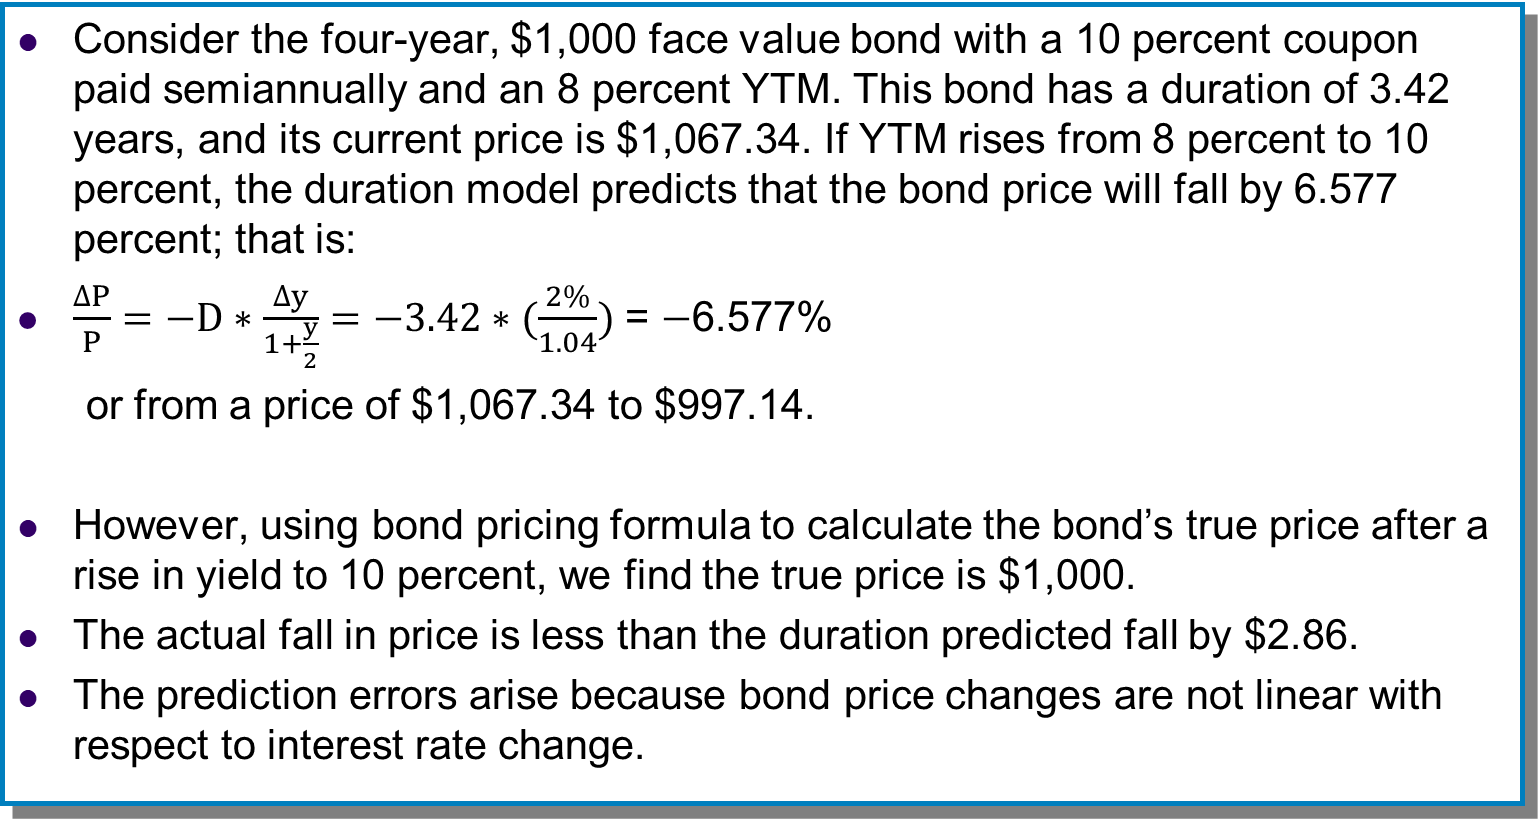
\includegraphics[width=\linewidth,keepaspectratio]{figures/slide57_img_flat.png}
\end{figure}
\end{column}
\begin{column}{0.46\textwidth}
\begin{figure}
\centering
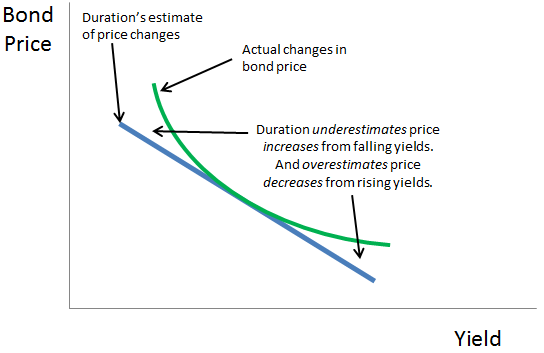
\includegraphics[width=\linewidth,keepaspectratio]{figures/slide58_img.png}
\end{figure}
\end{column}
\end{columns}
\end{frame}

% [src: 59]
\begin{frame}{Convexity}
The price--rate relationship is non-linear; \textbf{convexity (CX)} measures the change in the slope of the price--yield curve around rate level $R$, adding curvature to the duration estimate:
\[
\frac{\Delta P}{P} \approx -\,D \times \frac{\Delta y}{1+y} + \tfrac{1}{2}\,CX \times (\Delta y)^2
\]
\begin{itemize}
  \item The convexity term means the bond price is always \emph{above} the duration-model prediction
  \item Convexity is desirable: all else equal, more-convex bonds outperform less-convex bonds when yields move significantly in \emph{either} direction
\end{itemize}
\end{frame}

% ============ SUMMARY ============

% [src: 60]
\begin{frame}{Key Takeaways}
\begin{description}
  \item[Bond basics] Fixed-income securities promise a stream of cash flows. Key types: Treasury (default-free), municipal (tax-exempt), corporate (default risk)
  \item[Bond features] TIPS: principal adjusts with inflation, providing a real yield. Convertible: exchangeable for stock, lower yields. Callable: issuer redeems early, higher yields
  \item[Bond pricing and yields] Price $=$ PV of coupons $+$ PV of par (semi-annual discounting). Bond prices are \textbf{inversely} related to interest rates
  \item[Interest rate risk] Long-term and low-coupon bonds are most rate-sensitive. Duration measures average maturity and price sensitivity
\end{description}
\end{frame}

\end{document}
